\documentclass[11pt, a4paper]{article}

\usepackage[margin=0.6in]{geometry}
\usepackage{graphicx}
\usepackage{amsmath}
\usepackage{listings}
\usepackage{xcolor}
\usepackage{csquotes}
\usepackage{subfig}
\usepackage{url}
\usepackage{float}
\usepackage[hidelinks]{hyperref}


\definecolor{codegreen}{rgb}{0,0.6,0}
\definecolor{codegray}{rgb}{0.5,0.5,0.5}
\definecolor{codepurple}{rgb}{0.58,0,0.82}
\definecolor{backcolour}{rgb}{0.95,0.95,0.92}

\lstdefinestyle{mystyle}{
    backgroundcolor=\color{backcolour},
    commentstyle=\color{codegreen},
    keywordstyle=\color{magenta},
    numberstyle=\tiny\color{codegray},
    stringstyle=\color{codepurple},
    basicstyle=\ttfamily\small,
    breakatwhitespace=false,
    breaklines=true,
    captionpos=b,
    keepspaces=true,
    numbers=left,
    numbersep=5pt,
    showspaces=false,
    showstringspaces=false,
    showtabs=false,
    tabsize=2,
    language=Python
}
\lstset{style=mystyle}

\hypersetup{
    colorlinks=true,
    linkcolor=blue,
    filecolor=magenta,
    urlcolor=cyan,
    pdftitle={Birds and Blocks: A 2-Player Pygame Challenge},
    pdfpagemode=UseNone,
    pdfauthor={Aadeshveer Singh}
}

\title{Birds and Blocks: A 2-Player Pygame Challenge}
\author{Aadeshveer Singh \\ 24B0926}
\date{\today}

\begin{document}

\maketitle
\thispagestyle{empty}


\newpage

\begin{abstract}
\noindent This report details the design, implementation, and features of \enquote{Birds and Blocks,} a two-player physics-based game developed using Python and Pygame-CE. Inspired by Angry Birds, it adapts the core concept into a competitive, turn-based format. The players aim to destroy each other's fortresses using projectiles with distinct abilities. The game features custom-implemented projectile physics, destructible blocks (wood, stone, glass), a strategic bird upgrade system, persistent ELO-based player ratings with a leaderboard, and a complete set of custom pixel art assets and sound effects. The result is a polished, functional game showcasing concepts in game development, physics simulation, and software design.
\end{abstract}

\newpage

\tableofcontents

\newpage

\section{Introduction}
The mobile game Angry Birds captivated players with its simple but addictive physics-based puzzle game play. This project \enquote{Birds and Blocks,} takes inspiration from this core mechanic but transforms it into a two-player turn-based competitive experience.

The primary objective was to develop a 1v1 fortress destruction game using Python and the Pygame Community Edition (\texttt{ Pygame-CE}) library. Key requirements included implementing realistic projectile physics without relying on external physics engines, creating distinct projectile types with unique interactions against different block materials (wood, stone, glass), managing game states, handling player turns, and defining win/loss conditions.

Beyond the basic requirements, this project incorporates several advanced features: a card-based bird upgrade system unlocking special abilities, a persistent ELO rating system with a leaderboard, a dynamic camera, extensive custom pixel art and sound effects, and a contextual tutorial system. This report provides a comprehensive overview.

\vspace{2cm}

\section{Modules Used}

The development of "Birds and Blocks" relied on several standard Python libraries and the Pygame-CE library.

\begin{itemize}
    \item \textbf{Pygame-CE:} The core game development library. Used for window creation, input handling, graphics rendering, audio playback, font management, and game loop timing. Essential for all interactive and multimedia aspects.

    \item \textbf{random:} Utilized for various non-deterministic elements including initial fortress block layout generation, particle effect variations, and background cloud placement.
    
    \item \textbf{math:} Essential for physics calculations (distance, velocity components), aiming trajectory prediction, and launch velocity scaling.
    
    \item \textbf{os:} Used for interacting with the file system, primarily for loading assets (\texttt{os.listdir}) and ensuring the existence of user data files (\texttt{os.mknod}).
    
    \item \textbf{sys:} Used specifically for properly terminating the application via \texttt{sys.exit()} when the quit event is detected, ensuring a clean exit, especially when running as a compiled executable. Details can be found in Appedix \ref{app:exit_handle}.

\end{itemize}

Adhering to project guidelines, no external physics libraries (e.g., Pymunk) were utilized; all physics simulations were implemented using standard Python and the \texttt{math} library.

\newpage

\section{Directory Structure}

The project follows a well-organized directory structure, separating code, assets, documentation, and persistent data:

\begin{lstlisting}[basicstyle=\scriptsize\ttfamily, frame=single, numbers=none, caption={Final Project Directory Structure}, label={lst:dir_structure_final}]
.
+-- Birds_and_blocks(windows).exe  # Compiled Windows executable
+-- assets/               # Contains all non-code game resources
|   +-- audio/            # Sound effects (.wav files)
|   +-- fonts/            # Custom font file (custom_font.ttf)
|   +-- images/           # All visual assets (.png)
|       +-- UI/           # UI elements (buttons, screens, icons)
|       +-- background/   # Background scene images
|       |   ... (etc.)
|       +-- projectiles/  # Bird sprites (all types, states, upgrades)
+-- scripts/              # Core Python source code modules
|   +-- __pycache__/      # Python bytecode cache (auto-generated)
|   +-- birds.py          # Bird class (physics, abilities, collision)
|   |   ... (other .py files) ...
|   +-- utils.py          # Utility functions (Animation class)
+-- user_data/            # Stores persistent data between sessions
|   +-- players.txt       # Plain text list of registered player names
|   +-- ratings.txt       # Plain text list of corresponding ELO ratings
+-- report/               # Contains documentation files
|   +-- images/           # Screenshots used specifically in the report
|   |   +-- main_menu.png
|   |   |   ... (other report images) ...
|   |   +-- upgrade.png
|   +-- report.pdf        # Compiled PDF version of this report
|   +-- report.tex        # LaTeX source file for this report
|   +-- references.bib    # BibTeX bibliography database file
+-- main.py               # Main executable script (entry point)
+-- rename.bash           # Utility script (optional)
\end{lstlisting}

This structure maintains a clear separation of concerns: operational game assets in \texttt{assets/}, Python logic in \texttt{scripts/}, persistent player data in \texttt{user\_data/}, and all report-related files neatly contained within \texttt{report/}. The main script \texttt{main.py} serves as the entry point for running from source, while the \texttt{.exe} provides a standalone distribution. Note that the executable expects the \texttt{assets/} and \texttt{user\_data/} directories to be present in its runtime directory.


\section{Running Instructions}

There are two primary ways to run the game: from the Python source code or using the pre-compiled Windows executable.

\subsection{Prerequisites (Running from Source)}

\begin{itemize}

    \item Python 3.x installed.
    
    \item Pygame Community Edition (\texttt{pygame-ce}) installed. Use pip:
        \begin{lstlisting}[numbers=none, frame=single, language=bash]
pip install Pygame-CE
        \end{lstlisting}

\end{itemize}

\subsection{Execution}

\subsubsection{Option 1: Running from Source}

\begin{enumerate}

    \item Open a terminal or command prompt.
    
    \item Navigate (\texttt{cd}) to the project's root directory (where \texttt{main.py} is located).
    
    \item Execute the main script:
        \begin{lstlisting}[numbers=none, frame=single, language=bash]
python main.py
        \end{lstlisting}

\end{enumerate}

\subsubsection{Option 2: Running the Executable (Windows)}

\begin{enumerate}

    \item Ensure the \texttt{assets/} and \texttt{user\_data/} folders are present in the same directory as the executable file (\texttt{Birds\_and\_blocks(windows).exe}).
    
    \item Double-click the \texttt{Birds and blocks(windows).exe} file to launch the game directly.\footnote{\textbf{Note:} Some antivirus programs may flag executables created with PyInstaller as potentially suspicious due to the way they unpack components during runtime. This is often a false positive for applications compiled from trusted source code like this project.}

\end{enumerate}

The executable was created using PyInstaller, bundling the Python interpreter and necessary libraries.

\subsection{Controls}
\label{sec:controls}

Controls are the same regardless of the execution method:

\begin{description}

    \item[Menu Navigation:] Left-click on-screen buttons.
    
    \item[Name Input:] Left-click player box, type name, press \texttt{Enter} or \texttt{Tab}.
    
    \item[Aiming/Firing:] Left-click and drag bird in slingshot. Release to fire.
    
    \item[Special Abilities:] Left-click mid-air (if bird upgraded $>$ Level 1).
    
    \item[Sound Toggle:] Left-click speaker icon (top-left).
    
    \item[Back:] Left-click back arrow icon to return to menu.(Disabled in tutorial)
    
    \item[Exit:] Use window close button or detect \texttt{pygame.QUIT} event (handled internally via \texttt{sys.exit()}) to exit the application.

\end{description}


\section{Implemented Features}

This project implements core mechanics and several advanced features.

\subsection{How to Play}
\label{sec:how_to_play}

The objective of "Birds and Blocks" is to be the first player to completely destroy the opponent's fortress structure using bird projectiles launched from a slingshot.

\begin{itemize}

    \item \textbf{Turns:} The game proceeds in alternating turns between Player 1 and Player 2.
    
    \item \textbf{Bird Selection:} At the start of your turn, available bird cards are displayed (typically at the top of the screen). Left-click on a card to select the bird for launching.
    
    \item \textbf{Aiming and Firing:} Left-click and drag the selected bird in your slingshot area. A trajectory preview will appear. Pulling farther increases launch power. Release the left mouse button to fire the bird towards the opponent's fortress. You can right-click while aiming to cancel the shot.
    
    \item \textbf{Special Abilities:} If a bird type has been upgraded (Level $>$ 1), you can activate its special ability by left-clicking anywhere while the bird is in mid-air (once per shot). See Section \ref{sec:upgrades} for ability details.
    
    \item \textbf{Winning:} The first player to destroy all blocks comprising their opponent's fortress wins the game. The game will then transition to the Game Over screen.
    
    \item \textbf{Upgrade Phase:} After players exhaust their initial set of bird cards, an upgrade phase occurs where players can choose cards to enhance their birds' abilities for subsequent rounds.

\end{itemize}
Refer to Section \ref{sec:controls} for detailed button mappings.




\subsection{Game Interface and Flow}

\begin{itemize}

    \item \textbf{Screens:} Includes Main Menu, Player Name Entry, Gameplay, Tutorial overlays, Leaderboard, and Game Over (Figures \ref{fig:main_menu_a}, \ref{fig:name_input_a}, \ref{fig:gameplay_a}, \ref{fig:game_over_a}, \ref{fig:tutorial_a}, \ref{fig:leaderboard_a}).
    
    \item \textbf{State Management:} Game flow controlled by state variables in \texttt{main.py}.
    
    \item \textbf{UI Elements:} Custom buttons, indicators (turn, upgrade levels), text rendering using custom fonts handled by classes in \texttt{scripts/modes.py}.
    
    \item \textbf{Turn Structure:} Alternating turns managed in the main game loop.

\end{itemize}

\subsubsection{Game Fairness Considerations}

Several design choices aim to provide a fair competitive experience:

\begin{itemize}
    
    \item \textbf{Fortress:} The core map layout places both players' fortresses and slingshots symmetrically. The blocks are same though in random order to make the game feel new every time and randomness takes care of unsymmetry.
        
    \item \textbf{Turn-Based Gameplay:} Strict alternation ensures players have equal action opportunities per round.
    
    \item \textbf{Upgrade Opportunity Balancing:} While Player 1 takes the first game turn, fairness in the upgrade system is addressed. When the upgrade phase begins, Player 2 is given the `first choice' from the available upgrade card options. Subsequent upgrade opportunities alternate between players. This specific mechanism aims to counterbalance any slight advantage gained from starting first.

\end{itemize}

These factors contribute to a balanced playing field where victory primarily depends on player skill in aiming, strategic bird/upgrade selection, and understanding projectile interactions.


\begin{figure}[H]

  \centering
  
  \subfloat[Main Menu]{\label{fig:main_menu_a}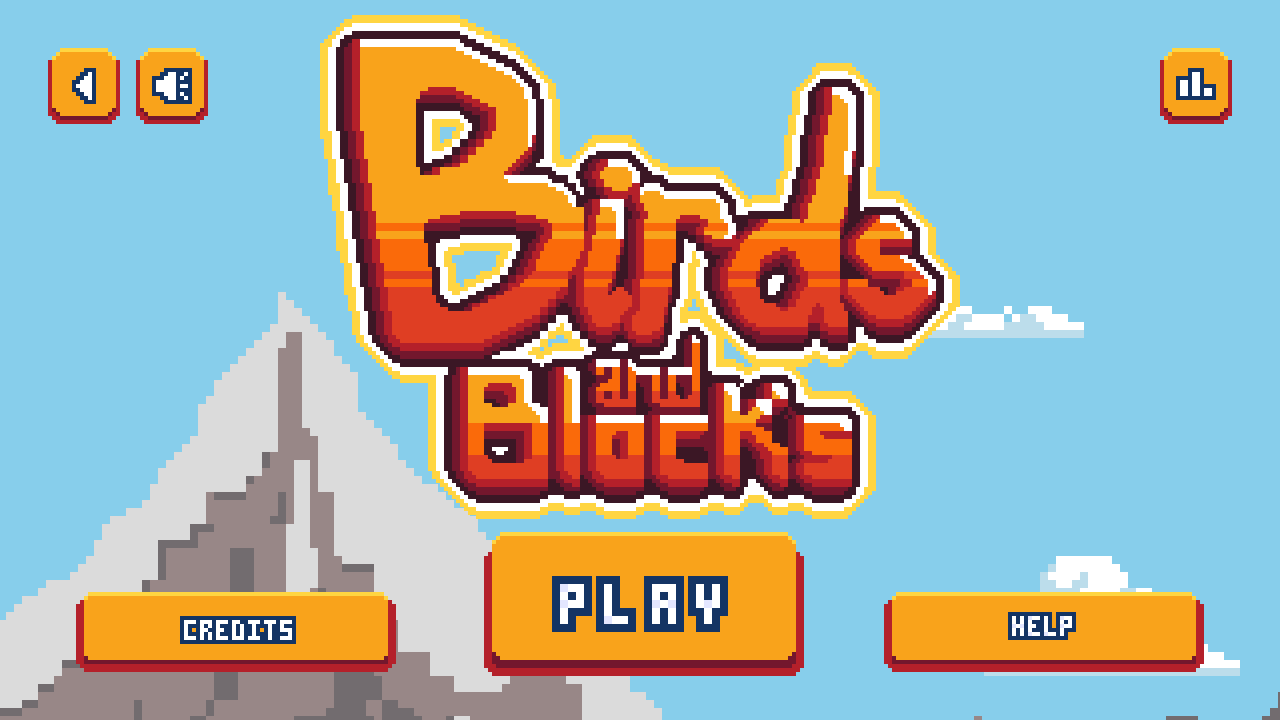
\includegraphics[width=0.48\textwidth]{images/main_menu.png}}
  \hfill
  \subfloat[Player Name Input]{\label{fig:name_input_a}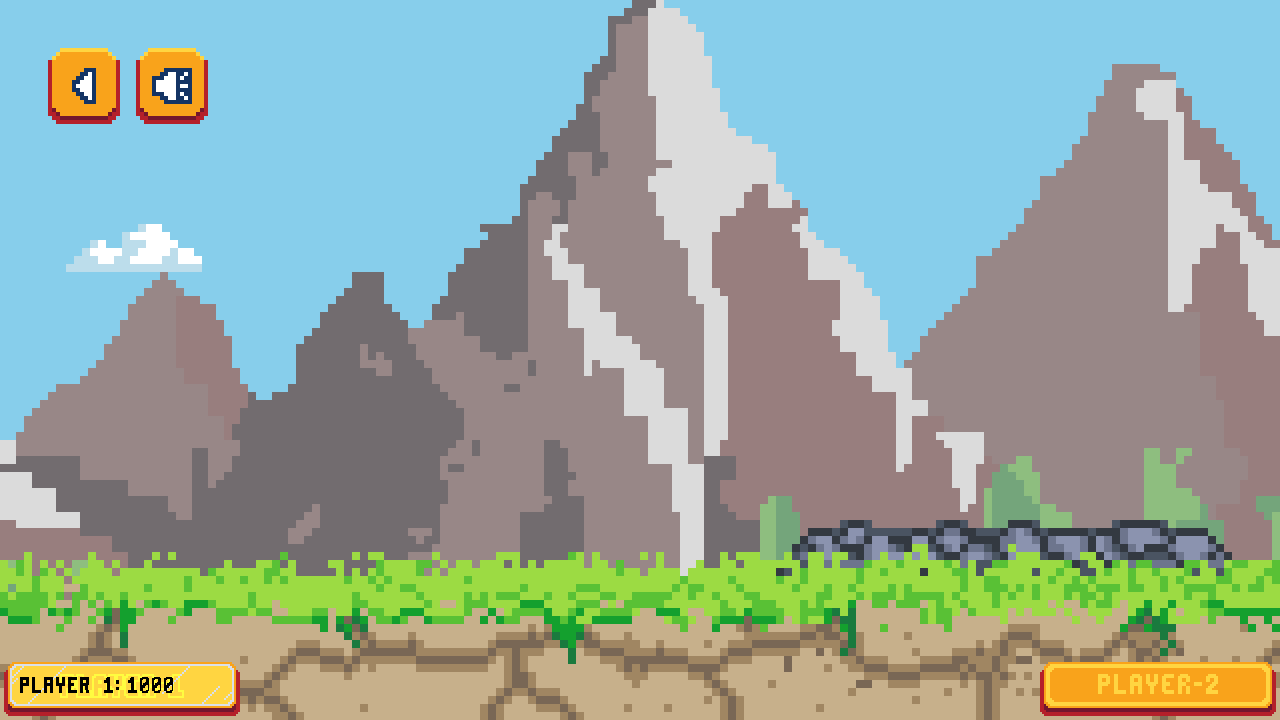
\includegraphics[width=0.48\textwidth]{images/name_input.png}}
  
  \vspace{1em}
  
  \subfloat[Gameplay Screen]{\label{fig:gameplay_a}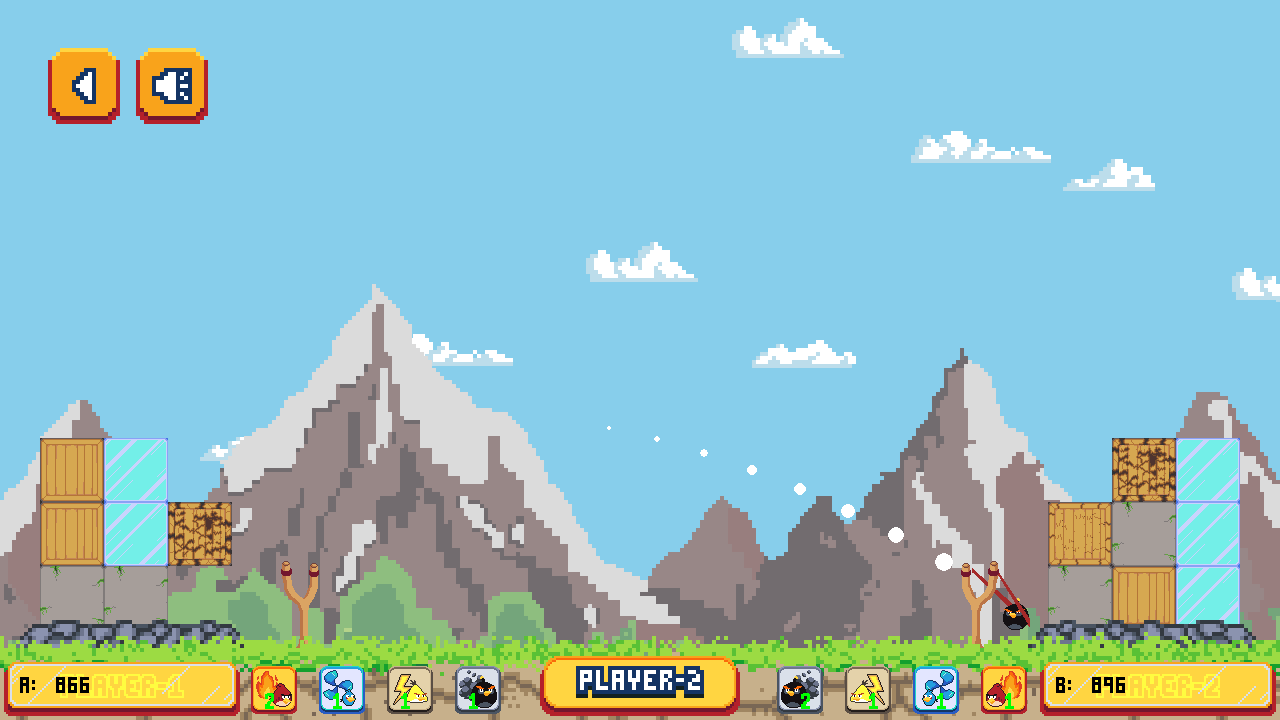
\includegraphics[width=0.48\textwidth]{images/game_play.png}}
  \hfill
  \subfloat[Game Over Screen]{\label{fig:game_over_a}
\includegraphics[width=0.48\textwidth]{images/game_over.png}}
  
  \caption{Key UI Screens Overview}
  
  \label{fig:ui_overview_a}

\end{figure}

\subsection{Core Gameplay Mechanics}

\begin{itemize}

    \item \textbf{Slingshot Physics:} Mouse drag calculates initial velocity based on distance and angle relative to the slingshot origin. Maximum speed is capped asymptotically (\texttt{scripts/birds.py}).
    
    \[\vec{v}=v_{max}(1-e^{-|\vec{r}|})\cdot\hat{r}\]
    
    Where, $v_{max}$ is set to $14$ and $\vec{r}$ is the cursor position vector relative to the slingshot origin.
    
    \item \textbf{Trajectory Preview:} Dots predict the flight path based on current launch parameters (\texttt{Bird.render}).
    
    \item \textbf{Projectile Motion:} Custom physics loop in \texttt{Bird.calculate\_next\_pos} updates position using current velocity and applies gravity (\texttt{GRAVITY = 1/6} equivalent to 1 unit per second as FPS = 60).
    
    \item \textbf{Collision Detection:} Bird's hitbox corners are checked against the opponent's block grid. Damage applied on hit (\texttt{Bird.collision\_check}).

\end{itemize}

\vspace{1cm}

\subsection{Projectiles (Birds)}
\label{sec:projectiles}

Four types implemented in \texttt{scripts/birds.py}: Red (balanced), yellow (versus wood), black (versus stone), and blue (versus glass). Damage calculation in \texttt{Bird.damage} includes base damage, speed factor, and type effectiveness multiplier.

\[\text{Damage}=(c_1+c_2\cdot|\vec{v}|)\cdot t\cdot u\]

Where $c_1$ and $c_2$ are constants for birds, $\vec{v}$ is the velocity vector and $t$ is the type multiplier and $u$ is the upgrade multiplier(\texttt{damage\_factor}) decided based on bird level and use. $t=1.5$ if type of bird is same as block it is about to hit, else $t=0.7$.

\begin{center}
    
    \begin{tabular}{|c||c|c|c|c|c|}
    
        \hline    
        \textbf{Projectile(Bird)}   & \textbf{$c_1$} & \textbf{$c_2$} & \textbf{Type} & \textbf{Special ability}\\
        \hline
        \textbf{Red}   & 35\footnotemark & 2 & Basic & Triple damage\\
        \hline
        \textbf{Blue}  & 20 & 2 & Glass & Splits into 3 identical projectiles\\
        \hline
        \textbf{Chuck} & 20 & 2 & Wood & Gets a speed boost\\
        \hline
        \textbf{Bomb}  & 20 & 2 & Stone & Blasts to do Area damage\\
        \hline

    \end{tabular}
        
\end{center}

\footnotetext{Red always induces $t=0.7$ hence absolute damage of red is higher to compensate.}

\vspace{1cm}

\subsection{Fortress (Blocks)}

Managed by \texttt{scripts/blockmap.py}:

\begin{itemize}

    \item \textbf{Types:} Wood, Stone, Glass with distinct health (\texttt{HEALTH\_MAP}).
    
    \begin{center}
        
        \begin{tabular}{|c|c|}
    
            \hline
            \textbf{Block type} & \textbf{Health} \\
            \hline
            \textbf{Glass} & 55\\
            \hline
            \textbf{Wood} & 75\\
            \hline
            \textbf{Stone} & 95\\
            \hline
        
        \end{tabular}
    
    \end{center}
    
    \item \textbf{Destruction:} HP reduced by bird impact damage.
    
    \item \textbf{Visual Damage:} 5-stage visual degradation based on remaining HP (Fig. \ref{fig:block_damage_a}).
    
    \item \textbf{Structure:} Grid-based; blocks currently float if support is removed.
    
    \item \textbf{Generation:} Randomly generated to introduce a new random element in every gameplay.

\end{itemize}

\begin{figure}[h!]

    \centering
    
    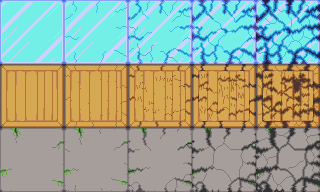
\includegraphics[width=0.7\textwidth]{images/block_damage.png}
    
    \caption{Visual Damage States for Blocks}
    
    \label{fig:block_damage_a}

\end{figure}

\vspace{1cm}

\subsection{Card \& Upgrade System}
\label{sec:upgrades}

Introduces strategic depth (\texttt{scripts/cards.py}, \texttt{scripts/player.py}):

\begin{itemize}

    \item \textbf{Flow:} Players choose bird cards, then upgrade cards after exhausting birds.
    
    \item \textbf{Abilities\footnote{More about special abilities and damage can be seen in section \ref{sec:projectiles}.} (Level $>$ 1):} Activated mid-flight via click: 
    
    \begin{description}
    
        \item[Red] (Damage+)
        
        \item[Yellow] (Speed++)
        
        \item[Blue] (Split)
        
        \item[Black] (Explosive area damage)
    
    \end{description}
    
    Implemented in \texttt{Bird.calculate\_next\_pos}.
    
    \item \textbf{UI:} Upgrade levels shown via icons (Fig. \ref{fig:upgrades_a}).

\end{itemize}


\begin{figure}[h!]

    \centering
    
    
\includegraphics[width=0.7\textwidth]{images/upgrade.png}
    
    \caption{Upgrade Indicators and Card Selection Example}
    
    \label{fig:upgrades_a}

\end{figure}

\vspace{1cm}

\subsection{ELO Rating System}

Persistent ranking (\texttt{scripts/rating.py}):

\begin{itemize}

    \item \textbf{Algorithm:} Standard ELO calculation (\texttt{ELO.update\_rating}).

    Expected score of player $a$ is give by:

    \[E_a = \frac{1}{1+10^{(R_b-R_a)/400}}\]

    Expected score of player $b$ is give by:

    \[E_b = \frac{1}{1+10^{(R_b-R_a)/400}}\]

    Where $R_a$ is rating of player $a$ and $R_b$ is rating of player $b$.
    After a match the winner scores $1$ point and loser scores $0$ points.
    This can be used to calculate new rating $R_{new} = R_{old} + 32(\text{Score}-\text{Expected score})$
    
    \item \textbf{Persistence:} Ratings stored in \texttt{user\_data/} text files. Two different files are used to store rating as using a single file(like \texttt{csv}) might cause problems if the user name has some special character.
    
    \item \textbf{Integration:} Displayed in name input and game over screens. Players ELO rating can be accessed by simply playing and inputting the name, the name will automatically turn to format \texttt{<user\_name> :<ELO>}. Top 9 players and their ratings can also be accessed through the leaderboard.

\end{itemize}

\vspace{1cm}

\subsection{Visuals and Audio}

Custom assets provide a unique identity:

\begin{itemize}

    \item \textbf{Pixel Art:} All visuals created by hand \texttt{pixel by pixel} using Aseprite software.
    
    \item \textbf{Sounds:} Custom \texttt{.wav} effects for actions; background music loop.
    
    \item \textbf{Particles:} Effects for feathers, dust, shards (\texttt{scripts/particles.py}). See Appendix \ref{app:particles} for implementation details.
    
    \item \textbf{Dynamic Camera:} Zooms/pans to follow projectiles.
    
    \item \textbf{Animations:} Used for birds, UI, clouds (\texttt{Animation} class). Appendix \ref{app:animation} provides details on its implementation.

\end{itemize}

\vspace{1cm}

\subsection{Dynamic Tutorial/Help}

Contextual guidance (\texttt{scripts/modes.py}):

\begin{itemize}

    \item \textbf{System:} Displays overlay images based on game state (\texttt{Tutorial} class).
    
    \item \textbf{Guidance:} Assists players through different phases (Fig. \ref{fig:tutorial_a}).

\end{itemize}

\begin{figure}[h!]

    \centering
    
    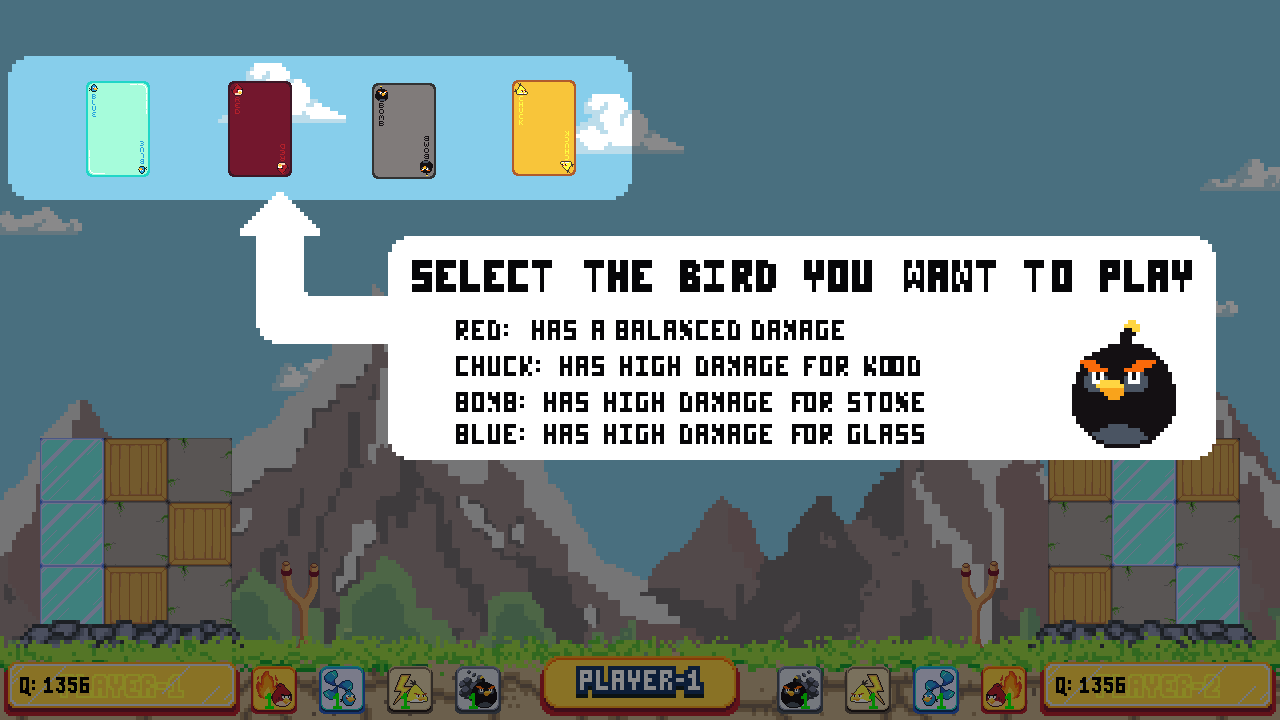
\includegraphics[width=0.7\textwidth]{images/tutorial.png}
    
    \caption{Dynamic Tutorial Overlay}
    
    \label{fig:tutorial_a}

\end{figure}

\newpage

\subsection{Leaderboard}

Displays player rankings:

\begin{itemize}

    \item \textbf{Access:} Button on main menu(Fig. \ref{fig:main_menu_a}).
    
    \item \textbf{Display:} Shows top players sorted by ELO (Fig. \ref{fig:leaderboard_a}).

\end{itemize}

\begin{figure}[h!]

    \centering
    
    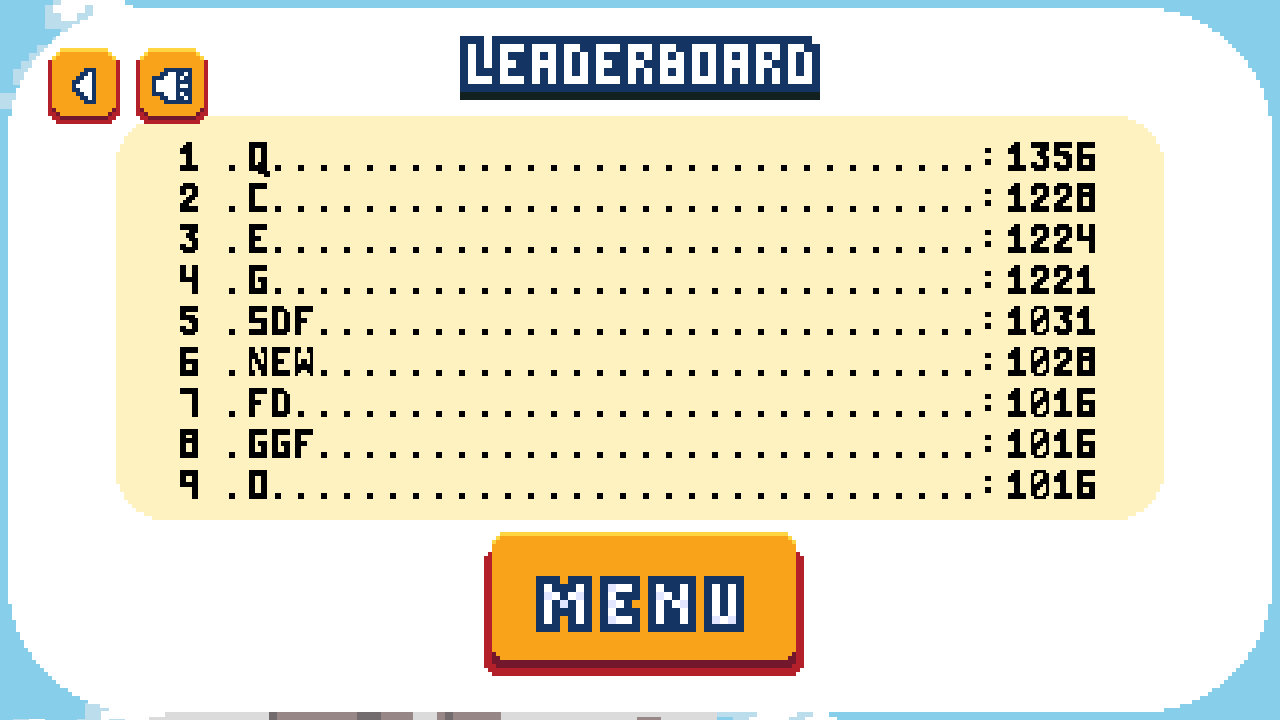
\includegraphics[width=0.7\textwidth]{images/leaderboard.png}
    
    \caption{Leaderboard Screen}
    
    \label{fig:leaderboard_a}

\end{figure}

\newpage

\section{Project Journey}

\subsection{Learnings}

Development involved learning Pygame-CE, game loop/state management, OOP design, custom physics simulation, asset management pipelines (Aseprite to Pygame), UI implementation, animation systems, and data persistence with file I/O for the ELO system.

\subsection{Challenges}

Major hurdles included tuning the custom physics and damage factors for intuitive gameplay, the extensive time required for custom pixel art creation, adding special visual effects efficiently, balancing the bird abilities and block health, managing complex state transitions smoothly, implementing a non-jarring dynamic camera, and ensuring the ELO system handled file operations robustly.

\subsection{Solutions}

These challenges were addressed through iterative testing and refinement cycles, a modular code structure enabled by OOP (using separate scripts), careful state definition and transition logic, extensive code commenting for clarity, using external tools like Aseprite efficiently for asset creation, and prioritizing core gameplay feel in physics implementation. Refactoring, like creating \texttt{loader.py}, also improved organization. Proper version management using Git and GitHub was employed throughout development. Finally, PyInstaller was used to package the game into a standalone executable for easier distribution on Windows.


\section{Conclusion}

\enquote{Birds and Blocks} successfully fulfills the project requirements by implementing a two-player physics-based game with custom mechanics using Pygame-CE. The inclusion of advanced features like the upgrade system, ELO ratings, leaderboard, dynamic camera, extensive custom assets, and an interactive tutorial significantly enhances the player experience, resulting in a polished and engaging final product. The project effectively demonstrates competence in various aspects of game development within the given constraints.

\newpage

\appendix

\section{Particle System Implementation Details}
\label{app:particles}

The game utilizes a particle system (\texttt{scripts/particles.py}) for various visual effects like feathers, dust, and block shards. This system consists of a \texttt{Particles} manager class that holds and updates a list of individual \texttt{Particle} objects. This appendix details the implementation of the core \texttt{Particle} class itself, which manages the state and movement of each visual effect element.

\subsection{The \texttt{Particle} Class}

This class represents a single visual effect particle, managing its state and movement.

\subsubsection{Initialization (\texttt{\_\_init\_\_})}

A particle is created with specific attributes:

\begin{lstlisting}[caption={Particle Class \_\_init\_\_ Snippet}, label={lst:particle_init_short}]
# From scripts/particles.py
class Particle:
    def __init__(self, animation, window_size, type, pos, vx, vy=1, 
                 effects=None, idx=None):
        self.anim = animation.copy() # Independent animation state
        self.pos = list(pos)         # Initial position
        self.vx, self.vy = vx, vy    # Initial velocity
        self.effects = effects if effects else [] # Behaviour modifiers
        # ... other setup like initial frame ...
\end{lstlisting}

Key initialization aspects:

\begin{itemize}

    \item Takes an \texttt{Animation} object for its visual frames.
    
    \item Sets initial position and velocity.
    
    \item The \texttt{effects} list (e.g., \texttt{'gravity', 'radial', 'sequence', 'cloud', 'fast'}) dictates behaviour modifications like applying gravity, randomizing velocity/position, controlling lifespan, or altering speed.

\end{itemize}

\subsubsection{Update Logic (\texttt{update})}

Called each game frame to update the particle's state:

\begin{lstlisting}[caption={Particle.update() Core Logic}, label={lst:particle_update_short}]
# From scripts/particles.py
def update(self):
    # Update position
    self.pos[0] += self.vx
    self.pos[1] += self.vy # + Potential 'float' effect variation

    # Apply effects like gravity
    if 'gravity' in self.effects:
        self.vy += 0.2 # Adjust gravity value as needed

    # Check lifespan: depends on effects
    if 'sequence' in self.effects:
        # Example: Remove if off-screen left (except clouds)
        finished = self.pos[0] < -self.anim.img().get_width()
        if finished and 'cloud' in self.effects:
            # Reset cloud position for looping effect
            # ... reset logic ...
            return False # Clouds don't "finish" this way
        return finished
    else:
        # Standard particles finish when their animation ends
        return self.anim.update()
\end{lstlisting}

The method updates position based on velocity, applies effects like gravity, and determines if the particle's lifecycle is complete (based on animation finishing or other conditions like going off-screen for sequence-based effects). It returns \texttt{True} when the particle should be removed.

\subsubsection{Rendering (\texttt{render})}

Simply draws the particle's current animation frame at its position:

\begin{lstlisting}[caption={Particle.render() Method}, label={lst:particle_render_short}]
# From scripts/particles.py
def render(self, surf):
    surf.blit(self.anim.img(), self.pos)
\end{lstlisting}

This system allows for flexible creation of various visual effects by combining different animations and behavioural flags.

\section{Animation Class Implementation}
\label{app:animation}

To handle multi-frame sprite animations consistently across different game objects (birds, blocks, UI elements, particles), a dedicated \texttt{Animation} class is implemented in \texttt{scripts/utils.py}. This class encapsulates animation data and logic, separating it from the game objects themselves.

\subsection{Purpose and Usage}

The primary goal is to manage a sequence of images (frames) and cycle through them over time based on a specified duration per frame. Game objects hold an instance of this class for their visual representation. Example usage when initializing a game object:
\texttt{self.anim = self.game.assets['projectile']['basic']['idle'].copy()}

\subsection{Class Implementation}

\subsubsection{Initialization (\texttt{\_\_init\_\_})}

Sets up the animation instance:

\begin{lstlisting}[caption={Animation Class \_\_init\_\_ Snippet}, label={lst:animation_init}]
# From scripts/utils.py
class Animation:
    def __init__(self, images, img_dur=5, loop=True):
        self.images = images        # List of pygame.Surface frames
        self.img_dur = img_dur      # How many game frames each image lasts
        self.loop = loop            # Whether the animation repeats
        self.frame = 0              # Internal counter tracking progress
        self.done = False           # Flag for non-looping animations
        self.length = len(images)   # Number of images in the sequence
\end{lstlisting}

\subsubsection{Updating State (\texttt{update})}

This method is called once per game frame to advance the animation:

\begin{lstlisting}[caption={Animation.update() Logic}, label={lst:animation_update}]
# From scripts/utils.py
def update(self):
    if self.loop:
        # Increment frame counter and loop using modulo
        self.frame = (self.frame + 1) % (self.length * self.img_dur)
    else:
        # Increment frame counter only if not done
        if not self.done:
            self.frame += 1
            # Check if end of animation reached
            if self.frame >= self.length * self.img_dur:
                self.done = True
    # Return True if a non-looping animation has finished
    return self.done
\end{lstlisting}

It increments an internal frame counter. If looping, it wraps around using the modulo operator. If not looping, it stops incrementing and sets the \texttt{done} flag when the end is reached. It returns the \texttt{done} status, useful for triggering events upon animation completion (like removing finished particles).

\subsubsection{Getting Current Image (\texttt{img})}

Calculates and returns the correct image surface for the current frame:

\begin{lstlisting}[caption={Animation.img() Method}, label={lst:animation_img}]
# From scripts/utils.py
def img(self):
    # Calculate the index into the images list
    image_index = int(self.frame / self.img_dur)
    return self.images[image_index]
\end{lstlisting}

This method is called by the game object's render method to draw the appropriate frame.

\subsubsection{Utility Methods}

\begin{itemize}

    \item \textbf{\texttt{copy()}:} Creates a new instance of the \texttt{Animation} with the same images and settings but with its own independent \texttt{frame} counter and \texttt{done} status. This is crucial so that multiple game objects using the same animation sequence (e.g., multiple identical particles) animate independently.
    
    \item \textbf{\texttt{set\_frame(frame)}:} Allows manually setting the internal \texttt{frame} counter, useful for synchronizing animations or resetting them to a specific state (e.g., setting block damage appearance).
    
    \item \textbf{\texttt{get\_frame()}:} Returns the current value of the internal \texttt{frame} counter.

\end{itemize}

This class provides a simple yet effective mechanism for managing sprite animations throughout the "Birds and Blocks" project.


\section{Application Exit Handling}
\label{app:exit_handle}

Proper application termination, especially for compiled executables, is handled using the \texttt{sys} module. The event loop checks for the \texttt{pygame.QUIT} event (typically triggered by closing the window) and calls \texttt{sys.exit()}.

\begin{lstlisting}[caption={Handling Quit Event in main.py}, label={lst:exit_logic}]
# Inside the main event loop (in game.run)
import sys # Ensure sys is imported at the top of main.py

# ... inside the 'for event in pygame.event.get():' loop ...
if event.type == pygame.QUIT:
    pygame.quit() # Uninitialize pygame modules
    sys.exit()    # Terminate the Python process cleanly
    # return # Or use return if in an async function context
# ... rest of event handling ...
\end{lstlisting}

Using \texttt{pygame.quit()} first is recommended to allow Pygame to clean up its resources before the script exits via \texttt{sys.exit()}.

\newpage


\section*{Bibliography / References / Resources Used}

\begin{itemize}

    \item Pygame Community Edition Official Website and Documentation: \href{https://pyga.me/}{https://pyga.me/}
    
    \item Python 3 Documentation: \href{https://docs.python.org/3/}{https://docs.python.org/3/}
    
    \item Aseprite (Pixel Art Software): \href{https://www.aseprite.org/}{https://www.aseprite.org/} (Used for asset creation)
    
    \item Advanced Pygame tutorial by DaFluffyPotato \url{https://www.youtube.com/watch?v=2gABYM5M0ww&t=20017s}
    
    \item ELO Rating System (Conceptual understanding): \href{https://en.wikipedia.org/wiki/Elo_rating_system}{https://en.wikipedia.org/wiki/Elo\_rating\_system}
        
    \item Beginner Pygame tutorial by FreeCodeCamp \url{https://www.youtube.com/watch?v=FfWpgLFMI7w}
    
    \item Pixabay (Free stock sounds): \href{https://pixabay.com/}{https://pixabay.com/} (Used to find sound effects)

    \item Stack overflow(For resolving errors and debuggin) \href{https://stackoverflow.com/}{https://stackoverflow.com/}
    
\end{itemize}

\end{document}